\chapter{Introduction}

\paragraph*{}
This progress report aims to highlight the progress of our final project, \textbf{Collective Transport using Swarm Robotics}, with the evaluating criteria being the team individual contributions, as well as our pace in comparison to the ideal schedule. The ideal schedule can be represented by the project Gantt Chart (Figure \ref{fig:gantt_chart}).

\paragraph*{}
During this iteration of the project timeline, we are expected to have started working on \textbf{Hardware} (Task 2.1), \textbf{SLAM in Two Environments} (Task 2.2), and \textbf{Improved SLAM} (Task 2.3). However, there have been some changes along the roadmap as a result of altered requirements. We are instead debating the necessity of having an improved version of SLAM, seeing as simple SLAM may already be sufficient for our task. Additionally, we are making an early initiative to \textbf{Combine Individual Modules into a Single Proper Simulation} (Task 2.4), as well as kick off \textbf{Robot Formation} (Task 3.2) as an attempt towards a stronger Minimum Viable Prototype (MVP).

\begin{figure}[H]
    \centering
    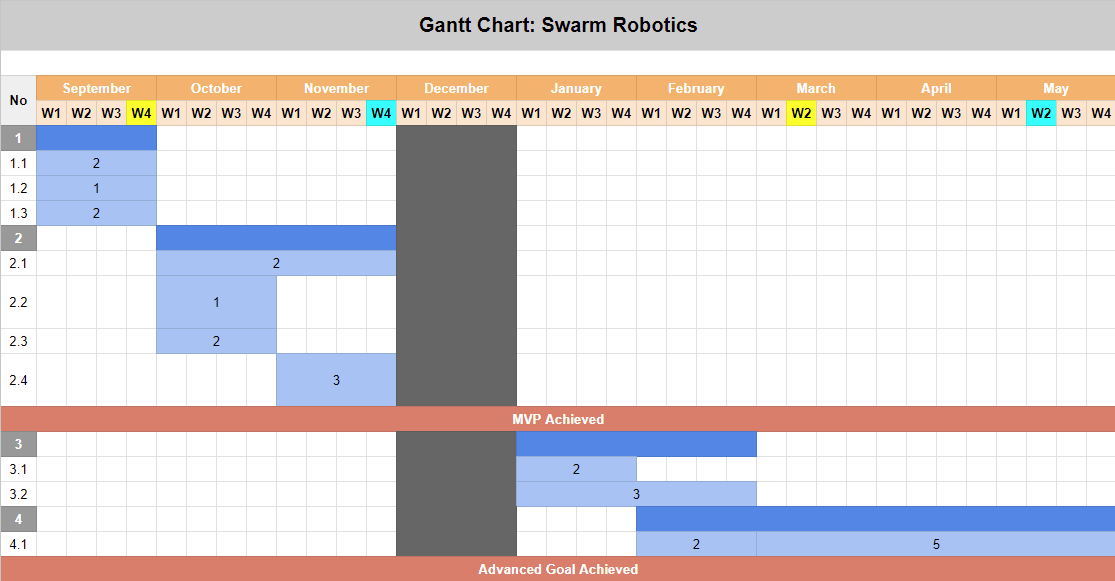
\includegraphics[width=1\linewidth]{assets/images/introduction/gantt_chart.png}
    \caption{Previous Project Gantt Chart}
    \label{fig:gantt_chart}
\end{figure}

\paragraph*{}
Thus, we are proposing an amendment to our project Gantt Chart to better align with our current requirements for our MVP (Figure \ref{fig:new_gantt_chart}). The main changes include listing the task \textbf{Simple Robot Formation} as Task 2.1, whereas \textbf{Hardware} has become a parallel effort and moved to Task 2.3. Moreover, \textbf{Combine Individual Modules in Simulation} (Task 2.4) has been modified to have already started. Furthermore, \textbf{Robot Formation} (Task 3.2) has been renamed \textbf{Advanced Robot Formation}. The differences between Simple Robot Formation and Advanced Robot Formation will be briefly described in the upcoming chapters.

\begin{figure}[H]
    \centering
    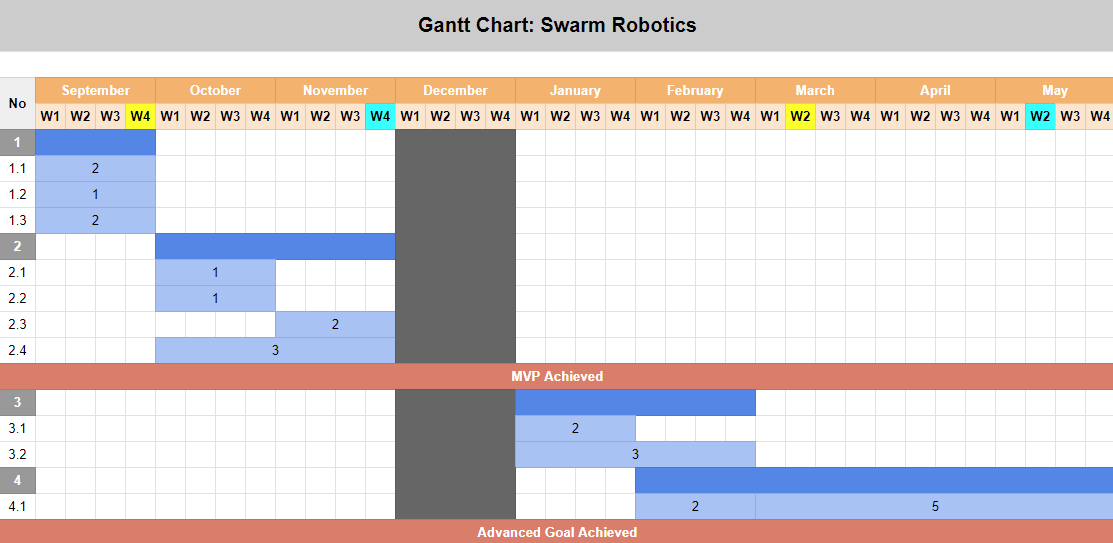
\includegraphics[width=1\linewidth]{assets/images/introduction/new_gantt_chart.png}
    \caption{New Project Gantt Chart}
    \label{fig:new_gantt_chart}
\end{figure}

\paragraph*{New Project Gantt Chart Task Outline:}
\begin{description}
    \item 1.1. Communication -- \textit{Completed}
    \item 1.2. Object Detection using Computer Vision -- \textit{Completed}
    \item 1.3. Simple Simultaneous Localization and Mapping -- \textit{In progress}
    \item 2.1. Simple Robot Formation -- \textit{In progress}
    \item 2.2. SLAM in two environments -- \textit{To do}
    \item 2.3. Hardware -- \textit{In progress}
    \item 2.4. Combine individual modules in simulation -- \textit{In progress}
    \item 3.1. Coordinated gripping -- \textit{To do}
    \item 3.2. Advanced Robot formation -- \textit{To do}
    \item 4.1. Hardware -- \textit{To do}
\end{description}
